\section{The Non-interacting Case}

For non-interacting particles, disabeling the Jastrow factor and forcing $\alpha=1$ provides the exact wave function for both quantum dots and atoms. In the case of molecules and the double-well, the additional requirement that $R\to\infty$ should also be applied. This serves as a powerful guide, since results can be benchmarked against exact solutions. In the non-interacting case, the minimization should always yield $\alpha=1$. 

The minimization method should seek an $\alpha$ close to one, where the variational derivative should be zero. The obtained energies should obey Eq.~(\ref{eq:qdotsE0}) in the case of quantum dots and Eq.~(\ref{eq:atomsE0}) in the case of atomic systems. In Table \ref{tab:res_valid_qdots}, validation runs for the three lowest closed-shell quantum dots are run for both two and three dimensions. Figure \ref{fig:ASGD_nonint} shows the ASGD method finding the minima. Table \ref{tab:res_valid_atoms} shows similar results for atoms.

The DMC method in case of an exact wave function should do nothing. The trial energy should equal the ground state energy through all time steps and zero fluctuations in the number of walkers should occur. This trend is shown for Neon in Fig. \ref{fig:DMC_neon_nonint}.

A final non-interacting case to run is the case of DMC without the exact wave function. As discussed in Chapter \ref{ch:QMC}, DMC should result in a better estimate of the ground state energy than VMC in case of a trial wave function different from the exact grouns state. A test-case is presented in Fig. \ref{fig:DMC_nonExactWF}.

\setlength{\tabcolsep}{0.3cm}
\begin{table}[h]
\begin{center}
\begin{tabular}{c|cccccc||cccccc}
 & & & 2D & & & & & & & 3D \\
\hline
  $\omega$   & N & $\mathrm{E_{VMC}}$ & $\mathrm{E_{DMC}}$ & $\alpha$ & $E_0$ & \qquad  & \qquad &  N   & $\mathrm{E_{VMC}}$ & $\mathrm{E_{DMC}}$ & $\alpha$ & $E_0$ \\
\hline
 0.5 &   2   &   1.0    &   1.0    &   1.0    & 1  & \qquad & \qquad & 2     &   3.0   &   3.0    &   1.0    & 3 \\
 1.0 &       &   2.0    &   2.0    &   1.0    & 2  & \qquad & \qquad &       &   1.5   &   1.5    &   1.0    & 1.5 \\
 0.5 &   6   &   5.0    &   5.0    &   1.0    & 5  & \qquad & \qquad &  8    &   18.0  &   18.0   &   1.0    & 18 \\
 1.0 &       &   10.0   &   10.0   &   1.0    & 10 & \qquad & \qquad &       &  9.0    &   9.0    &   1.0    & 9 \\
 0.5 &   12  &   14.0   &   14.0   &   1.0    & 14 & \qquad & \qquad & 20    &  60.0   &   60.0   &   1.0    & 60 \\
 1.0 &       &   28.0   &   28.0   &   1.0    & 28 & \qquad & \qquad &       &  30.0   &   30.0   &   1.0    & 30 \\
\end{tabular}
\caption{Validation results for quantum dots. The last column of each dimensions region lists the exact energies calculated from Eq.~(\ref{eq:qdotsE0}). }
\label{tab:res_valid_qdots}
\end{center}
\end{table}
\setlength{\tabcolsep}{6pt}

\setlength{\tabcolsep}{0.7cm}
\begin{table}[h]
\begin{center}
\begin{tabular}{cc|cccc}
  $\omega$   & N & $\mathrm{E_{VMC}}$ & $\mathrm{E_{DMC}}$ & $\alpha$ & $E_0(R\to\infty)$ \\
\hline
  0.5  &       &   4.0   & 4.0   &   1.0    & 4   \\
  1    &   4   &   2.0   & 2.0   &   1.0    & 2   \\
  0.5  &       &   20.0  & 20.0  &   1.0    & 20  \\
  1    &   12  &   10.0  & 10.0  &   1.0    & 10  \\
  0.5  &       &   28.0  & 28.0  &   1.0    & 28   \\
  1    &   24  &   56.0  & 56.0  &   1.0    & 56   \\
\end{tabular}
\caption{Validation results for double-well quantum dots. The exact energy is listed in the last column. The calculations are performed with the wells separated at a distance $R=20$.}
\label{tab:res_valid_qdots_doublewell}
\end{center}
\end{table}
\setlength{\tabcolsep}{6pt}

\setlength{\tabcolsep}{1cm}
\begin{table}
\begin{center}
\begin{tabular}{c|cccc}
    N     & $\mathrm{E_{VMC}}$ & $\mathrm{E_{DMC}}$ & $\alpha$ & $E_0$\\
\hline
    2     &   -4.0   &   -4.0   &   1.0  & -4  \\
    4     &  -20.0   &  -20.0   &   1.0  & -20 \\
    10    &  -200.0  &  -200.0  &   1.0  & -200\\
\end{tabular}
\caption{Validation results for Atoms. The exact energies $E_0$ are calculated from Eq.~(\ref{eq:atomsE0}).}
\label{tab:res_valid_atoms}
\end{center}
\end{table}
\setlength{\tabcolsep}{6pt}

\setlength{\tabcolsep}{0.8cm}
\begin{table}
\begin{center}
\begin{tabular}{c|cccc}
    N     & $R$ & $\mathrm{E_{VMC}}$ & $\mathrm{E_{DMC}}$ & $E_0(R\to\infty)$\\
\hline
    4     & 10  &   -8.403     &  -8.398    & -8  \\
          & 100 &   -8.085     &  -8.067    &     \\
          & 325 &   -8.032     &  -8.030    &     \\
    8     & 10  &  -41.596     &  -41.608   & -40 \\
          & 100 &  -40.298     &  -40.231   &     \\
          & 325 &  -40.123     &  -40.112   &     \\
    20    & 10  &  -409.999    &  -410.010  & -400\\
          & 100 &  -401.390    &  -401.049  &     \\
          & 325 &  -           &  -         &     \\
\end{tabular}
\caption{Validation results for Molecules. The last column lists the exact energies calculated from Eq.~(\ref{eq:atomsE0}). The energies converge to the exact energies, however, slower than the double well. Setting $R$ too high results in a singular slater determinant due to finite machine precision.}
\label{tab:res_valid_molecules}
\end{center}
\end{table}
\setlength{\tabcolsep}{6pt}


\begin{figure}[h]
 \begin{center}
  \subfigure{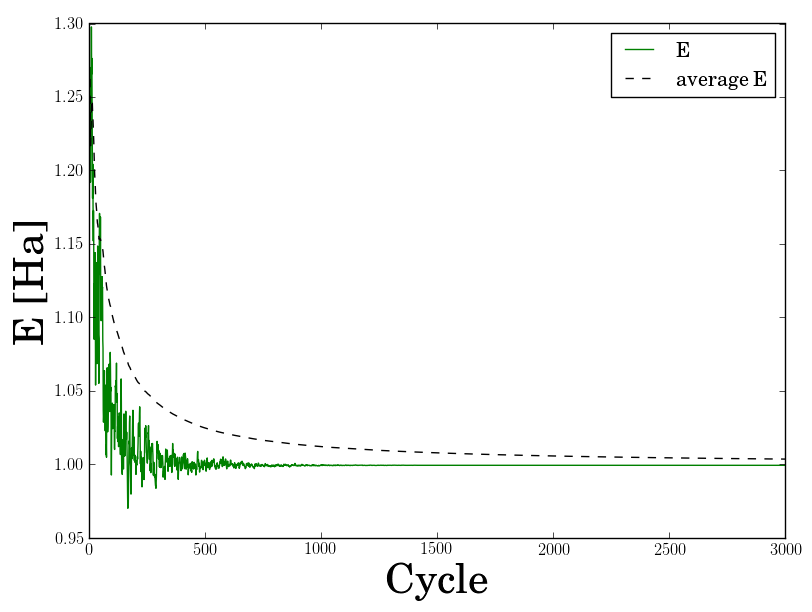
\includegraphics[scale=0.37]{../Graphics/ASGD_nonint_E.png}}
  \subfigure{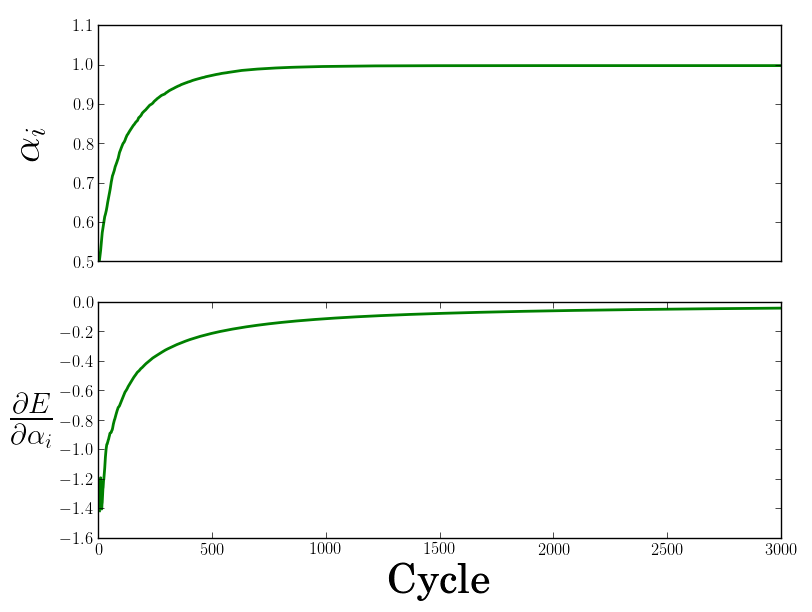
\includegraphics[scale=0.37]{../Graphics/ASGD_nonint.png}} 
  \caption{ASGD results for a non-interaction two-particle Quantum Dot with $\omega=0.5$. The exact energy of $E_0=1$ is reached after approximatly 1000 cycles, where $\alpha$ has converged close to unity. Due to enormous fluctuations, the variational derivative is plotted as an accumulated average, and is in practice dead zero after 1000 cycles. The variational principle described in Section \ref{sec:selectingOptVarPar} is governing the trend of the energy convergence, however, alot of statistical noise is present in the first 1000 cycles due to high variance and few samples.}
  \label{fig:ASGD_nonint}
 \end{center}
\end{figure}



\begin{figure}[h]
 \begin{center}
  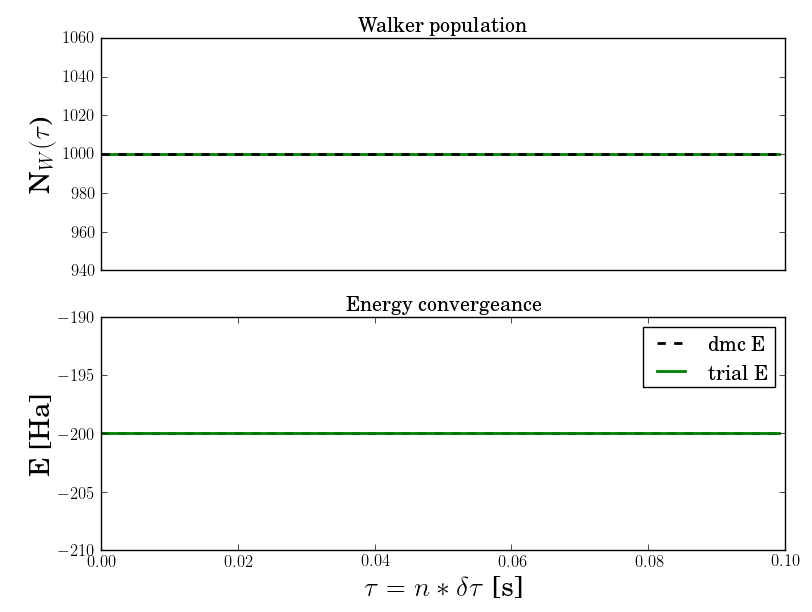
\includegraphics[scale=0.5]{../Graphics/DMC_neon_valid.png}
  \caption{DMC convergence for the Neon result listed in Table \ref{tab:res_valid_atoms}. The trial energy is fixed at the exact ground state energy as expected. The number of walkers are constant, implying a approximatly zero variance.}
  \label{fig:DMC_neon_nonint}
 \end{center}
\end{figure}

\begin{figure}[h]
 \begin{center}
  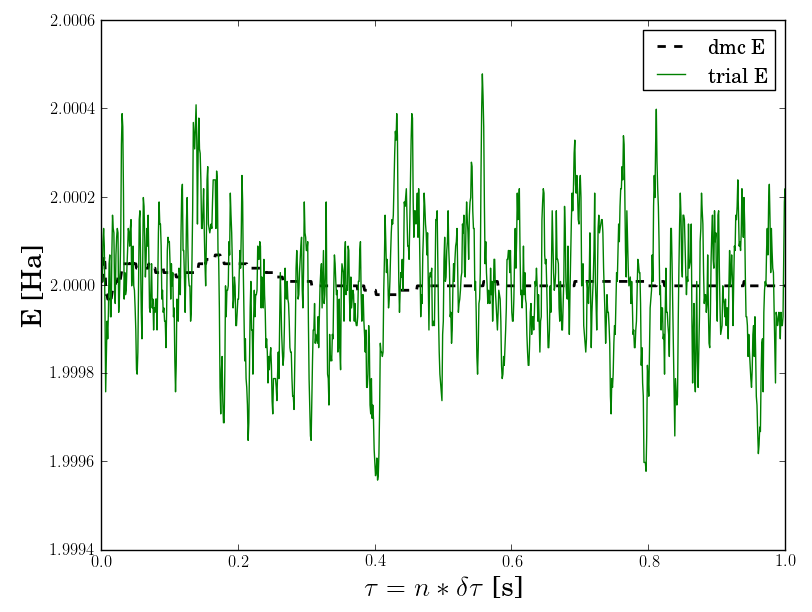
\includegraphics[scale=0.5]{../Graphics/DMC_notExactWF.png}
  \caption{DMC convergence for a non-interacting two-particle Quantum Dot with $\omega=1$. Calculations are done with $\alpha=0.75$, where the exact wave function is given for $\alpha=1$. Unlike the case with the exact wave function, the trial energy oscillates around the exact value. The final result (with blocking) reveals a DMC energy of $2.00000(2)$, where the original VMC energy was $2.0042(3)$. This illustrates the power of DMC over VMC in the interesting cases with an unknown exact wave function. The calculation were done with $10000$ walkers.}
  \label{fig:DMC_nonExactWF}
 \end{center}
\end{figure}